\chapter{Notes}

\section{Statistics}

\begin{itemize}
\item binominal density function can be approximated by Poisson density function when $np = \lambda$ is large, i.e. when $n \rightarrow \infty$ and $p \rightarrow 1$
\item log-normal distribution is skewed to the right (e.g. positively skewed) with
\begin{gather*}
f(x) = e^{\frac{1}{2}\sigma^2 - \mu} \frac{1}{\sigma \sqrt{2 \pi}} e^{-\frac{1}{2}\left(\frac{\ln x - (\mu - \sigma^2)}{\sigma}\right)^2}\\
E[X] = e^{\mu + \frac{1}{2}\sigma^2}\\
D[X] = (e^{\sigma^2} - 1)e^{2\mu + \sigma^2}
\end{gather*}
\item equatility of two population variances - assumes that the two populations are normally distributed; always construct F-statistics such that $s_1^2 > s_2^2$
\begin{equation*}
F_{n_1 - 1, n_2 - 1} = \frac{s_1^2}{s_2^2}
\end{equation*}
\item $A = \beta_1^A EQ + \beta_2^A BND$ and $B = \beta_1^B EQ + \beta_2^B BND$
\begin{equation*}
cov_{A,B} = \sum_{i,j}\beta_i, \beta_j \sigma_i \sigma_j = \beta_1^A \beta_1^B \sigma_{EQ}^2 + \beta_2^A \beta_2^B \sigma_{BND}^2 + \beta_1^A \beta_2^B cov_{EQ,BND} + \beta_2^A \beta_1^B cov_{EQ,BND}
\end{equation*}
\begin{figure}[htp]
\centering
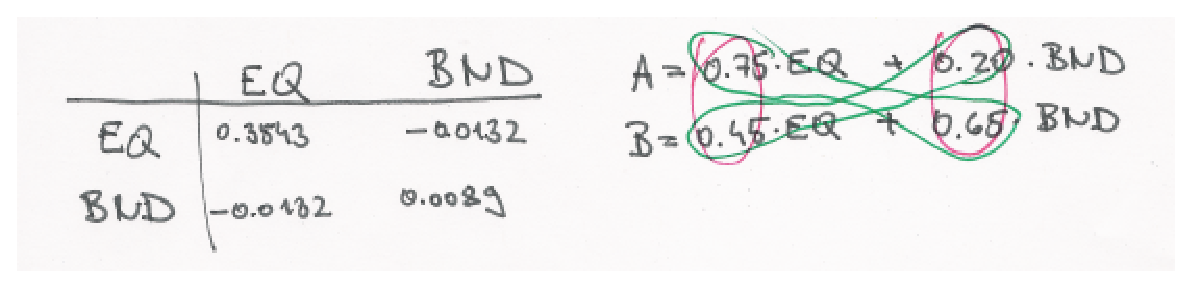
\includegraphics[scale = 0.75]{reg.eps}
\caption{covariance in regression model}
\label{reg}
\end{figure}
\item mixture distribution
\begin{gather*}
f(x; a_1, ..., a_n, b_1, ..., b_n) = \sum_i^n w_i p_i(x; a_i, b_i)\\
F(x; a_1, ..., a_n, b_1, ..., b_n) = \sum_i^n w_i F_i(x; a_i, b_i)
\end{gather*}
\item goodness-of-fit - chi-square and Kolmogorov-Smirnov test 
\end{itemize}

\section{Regression and OLS}

\begin{itemize}
\item Regardless homo/heteroskedasticity OLS estimator is unbiased, consistent and assymptotically normal. Homoskedasticity ensures that OLS estimators are efficient (i.e. the lowest volatility).
\item adjusted $R^2$ penalizes for number $k$ of slopes in the regression model
\begin{equation*}
\overline{R^2} = 1 - \frac{n - 1}{n - k - 1}R^2
\end{equation*}
\item standard error of regression
\begin{equation*}
SER = \sqrt{\frac{SSR}{n - k -1}}
\end{equation*}
\item confidence interval of $E[Y|X]$ could be calculated as $E[Y|X] \pm \Phi(\alpha/2)\sigma_{\epsilon}$
\begin{gather*}
Y = \beta_0 + \beta_1 X + \epsilon\\
E[Y|X] = \beta_0 + \beta_1 X
\end{gather*}
\item error term and independent variable have constant volatility
\item We have a linear model $Y = \beta_0 + \beta_1 X + \epsilon$. We know $\beta_1, \sigma^2_Y$ and $\sigma^2_{\epsilon}$. What is $\rho_{X,Y}$?
\begin{gather*}
\sigma_Y^2 = \beta_1^2 \sigma_X^2 + \sigma_{\epsilon}^2\\
\sigma_X^2 = \frac{\sigma_Y^2 - \sigma_{\epsilon}^2}{\beta_1^2}\\
\beta_1 = \rho_{X,Y} \frac{\sigma_Y}{\sigma_X}\\
\rho_{X,Y} = \frac{\beta_1 \sigma_X}{\sigma_Y}
\end{gather*}
\item homoskedasticity-only F-statistics
\begin{gather*}
F = \frac{(SSR_{rest} - SSR_{unrest}) / q}{SSR_{unrest} / (n - k - 1)}\\
F = \frac{(R^2_{unrest} - R^2_{rest}) / q}{(1 - R^2_{unrest}) / (n - k - 1)}
\end{gather*}
\end{itemize}

\section{EWMA, GARCH}

\begin{itemize}
\item GARCH model $\sigma_n^2 = \omega + \alpha u_{n-1}^2 + \beta \sigma_{n-1}^2$
\begin{itemize}
\item $u_{n-i}^2$ is weighted with $\alpha \beta^{i-1}$
\item persistence $\alpha + \beta$ - the larger the persistence the longer to revert to mean
\item volatility prediction $E[\sigma_{n+t}^2] = V_L + (\alpha + \beta)^t(\sigma_n^2 - V_L)$
\item mean reversion introduces autocorrelation into volatility estimates
\begin{itemize}
\item $VaR_{n-days} = VaR_{1-day}\sqrt{n + n\rho}$
\item if $\sigma_n^2 < V_L$ $\Rightarrow$ volatility is expected to grow $\Rightarrow$ positive autocorrelation $\Rightarrow$ square-root-of-time VaR underestimate the true VaR
\item if $\sigma_n^2 = V_L$ $\Rightarrow$ volatility is expected to be stable $\Rightarrow$ no autocorrelation $\Rightarrow$ square-root-of-time VaR is a good estimate of the true VaR
\item if $\sigma_n^2 > V_L$ $\Rightarrow$ volatility is expected to decrease $\Rightarrow$ negative autocorrelation $\Rightarrow$ square-root-of-time VaR overestimate the true VaR
\end{itemize}
\end{itemize}
\item EWMA model $\sigma_n^2 = \lambda \sigma_{n-1}^2 + (1-\lambda)u_{n-1}^2$
\begin{itemize}
\item $u_{n-i}^2$ is weighted with $(1-\lambda) \lambda^{i-1}$
\end{itemize}
\end{itemize}

\section{VaR}

\begin{itemize}
\item historical simulation VaR is not subjected to model risk vs. may not recognize changes in volatility and correlations from structural changes
\item VaR increases with increasing speed in quantile and increases with decreasing speed in holding period (the speed is inverse to expected gain on the underlying portfolio)
\item operational VaR - basic and standardized approach - only positive income is taken into account
\item expected credit loss: commitment = outstanding + (commitment - outstanding) * usage given default
\item bootstraping method of simulation - you randomly draw from historical data
\end{itemize}

\section{Ratings}

\begin{itemize}
\item ratings and quantitative scoring methods cannot be compared
\item default rates show statistically significant variations based on industry (vs. region)
\end{itemize}

\section{CAPM and Related Measures}

\begin{itemize}
\item $R_P = R_F + \beta(PR_{market} + PR_{country})$
\item expected rate of return vs rate of return implied by CAPM
\begin{figure}[htp]
\centering
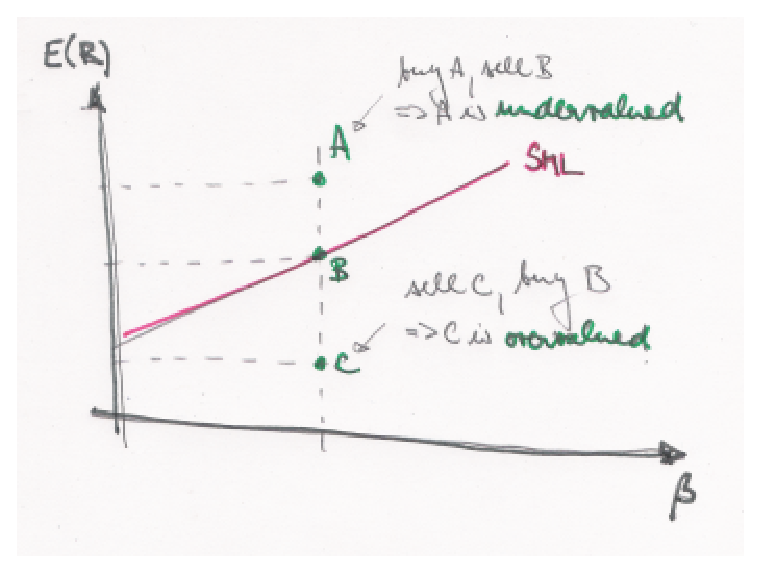
\includegraphics[scale = 0.75]{capm.eps}
\caption{CAPM}
\label{CAPM}
\end{figure}
\end{itemize}

\section{Bonds}

\begin{itemize}
\item government bonds are priced in 1/32; corporate and municipal bonds are priced in 1/8
\item numerical delta and gamma calculation
\begin{gather*}
D = \frac{1}{PV^0}\frac{PV^+ - PV^-}{\Delta y}\\
C = \frac{1}{PV^0}\frac{PV^+ + PV^- - 2PV^0}{(\Delta y)^2}
\end{gather*}
\item modified duration of ZCB is slightly lower than its maturity; Macaulay duration of ZCB equals its maturity
\item effective duration - takes into consideration changes in cash-flows resulting from changes in yield $\Rightarrow$ more convenient for bonds with embedded options (vs. modified duration)
\item perpetuity duration is $D = \frac{1}{y}$ $\Rightarrow$ does not depend on coupon
\item convexity grows with square of time and falls with coupon
\item duration is relative measure $\Rightarrow$ two bonds with the same duration but different NPV $\Rightarrow$ the same relative price change but different USD price change
\end{itemize}

\section{Mortgages}
\begin{itemize}
\item recourse loan - allows the lender to go after the debtor's assets that were not used as loan collateral in case of default
\end{itemize}

\section{Futures}

\begin{itemize}
\item order types
\begin{itemize}
\item market order - carried out immediately at current market price
\item limit order - executed at specified or more favorable price; waiting for low price to buy
\item stop order / stop-loss order - executed at specified or less favorable price; minimize loss
\item stop-limit order - current stock price is 50 USD, sell at 48 USD with limit of 47 USD $\Rightarrow$ conditional on bid or ask falling to 48 USD, sell order is is filled in if the sale can be exercised at 47 USD or higher (but may not be filled at all)
\item market-if-touched order - market order if a specified price is reached
\item discretionary / market-not-held order - market order with broker's discretion in an attempt to get a better price
\item time-of-day - specifies a particular time period of trading day
\item open order - can be executed during a given trading day
\item fill-or-kill - has to be executed immediately or not at all
\end{itemize}
\item hedge effectivness - proportion of variance eliminated by hedging
\begin{equation*}
effectivness = R^2 = \rho^2 = 1 - \frac{variation~of~basis}{variation~of~spot} = 1 - \frac{\sigma^2_{S - F}}{\sigma^2_S}
\end{equation*}
\item forward price adjustmend
\begin{equation*}
fwd = fut - \frac{1}{2}\rho \sigma^2 T_1 T_2
\end{equation*}
\item long Eurodolar futures position = short bond position
\item short hedge position, i.e. selling futures = long position in basis $\Rightarrow$ gain if basis streghtens
\begin{equation*}
BS = S_T - F_0
\end{equation*}
\end{itemize}

\section{Options}

\begin{itemize}
\item rho vs moneyness
\begin{figure}[htp]
\centering
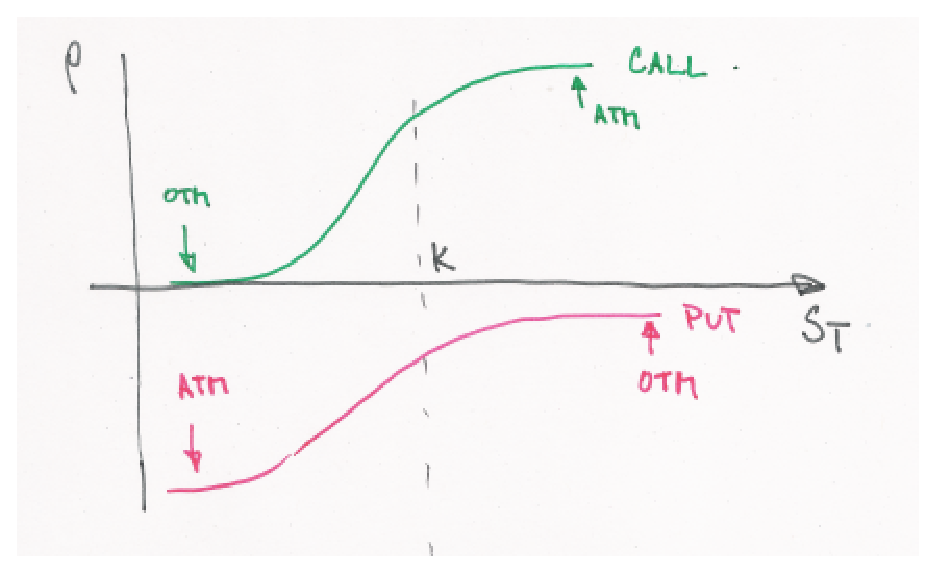
\includegraphics[scale = 0.75]{rho.eps}
\caption{rho}
\label{rho}
\end{figure}
\item American call can be exercised prior (not on) ex-dividend day
\item American call might be exercised for $q > r$ and small $T$
\item American put might be exercised if $q$ is small and $r$ increases (because stock prices tend to fall)
\item limits on option prices are
\begin{gather*}
max(S_T - Xe^{-rT}, 0)\le c \le S_0\\
max(S_T - Xe^{-rT}, 0)\le C \le S_0\\
max(Xe^{-rT} - S_T, 0)\le p \le X e^{-rT}\\
max(X - S_T, 0)\le P \le X
\end{gather*}
\item vega is the greatest for ATM options with long maturities
\item horizontal spread = calendar spread
\item collar
\begin{gather*}
collar = p - c\\
collar = covered~call~+~protective~put~=~p - c + S_0
\end{gather*}
\begin{figure}[htp]
\centering
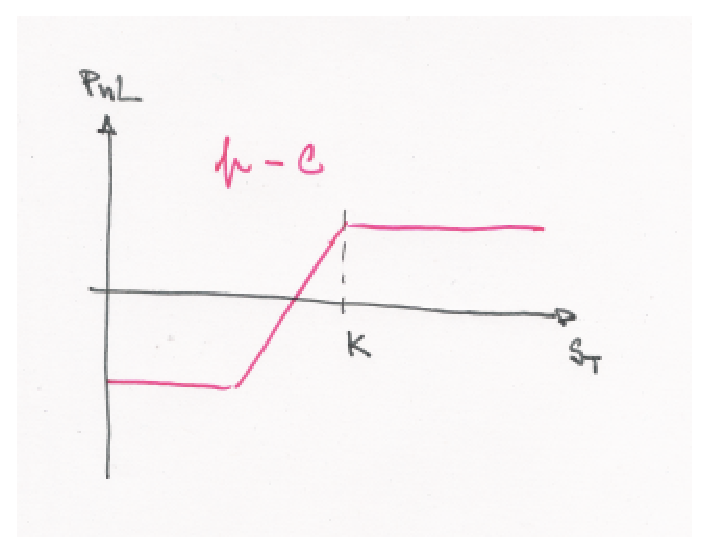
\includegraphics[scale = 0.75]{collar.eps}
\caption{collar}
\label{collar}
\end{figure}
\end{itemize}



